\documentclass[12pt, letterpaper]{article}

\usepackage[utf8]{inputenc}
\usepackage{mathtools}
\usepackage[left=0.6in, right=0.6in, top=1in, bottom=1in]{geometry}
\usepackage{graphicx}
\usepackage{algorithm}
\usepackage{algpseudocode}
% \usepackage{changepage}
\usepackage{xcolor}
\usepackage{amsmath}

% for code snippets
\usepackage{listings}
\usepackage{color}

\definecolor{dkgreen}{rgb}{0.5,0.65,0.5}
\definecolor{gray}{rgb}{0.5,0.5,0.5}
\definecolor{code_blue}{rgb}{0.10,0.27,0.92}
\definecolor{str_red}{rgb}{0.87,0.2,0.14}

\lstset{frame=tb,
  language=Java,
  aboveskip=3mm,
  belowskip=3mm,
  showstringspaces=false,
  columns=flexible,
  basicstyle={\small\ttfamily},
  numbers=none,
  numberstyle=\tiny\color{gray},
  keywordstyle=\color{code_blue},
  commentstyle=\color{dkgreen},
  stringstyle=\color{str_red},
  breaklines=true,
  breakatwhitespace=true,
  tabsize=3
}

\title{CSE 101 Homework 3}
\author{Kreshiv Chawla, Brian Masse, Taira Sakamoto, Emily Xie, Annabelle Coles}
\date{October 21, 2025}

\begin{document}

\maketitle
\newpage

\begin{enumerate}

% MARK: Question 1
%--------------------- Question 1 ---------------------
\item \textbf{Degrees of separation}

In the seven degrees of Kevin Bacon party game, you try to connect the actor Kevin Bacon to a challenge actor by giving a sequence of movies and actors, so that Kevin bacon and the first actor in the list were in the first movie on the list, the first actor and second actor on the list were in the second movie, and so on, and the last actor on the list was the one you were challenged. 

We can make this an algorithmic problem as follows.
We are given a list of movies, and for each movie, a list of actors that
appeared in the movie.  There are $M$ movies total, and the total length of all the lists for all movies is $L$. We are given actors $A$ and $B$ and want to find a list of pairs $(movie_1,actor_1),...(movie_k,actor_k=B)$ so that
both $A$ and $actor_1$ are in $movie_1$, and for
$i=2...k$, $actor_{i-1}$ and $actor_i$ are
both in $movie_i$.  We want to make the number of movies $k$ as small as possible.  

Below, you will describe how to use a graph algorithm from class to solve the
problem.
\begin{enumerate}
\item  What graph will you use to solve the problem?  Be sure to specify the set of vertices in your graph, the set of edges, whether the edges are directed or undirected, and what weights edges have, if any.  
(4 points )
\item How will you create the graph from the information given?  What format will you use for the graph?  How long does it take to create the graph?
(2 points)
\item How many vertices does your graph have, at most? Give this in terms of $M$ and $L$ 
(2 points)
\item How many edges does your graph have, at most? Give this in terms of $M$ and $L$ 
(2 points)
\item  How do paths in your graph relate to solutions for the degrees of separation problem?  What is the relationship between the length of paths and the number of movies $k$ in a corresponding solution?
(4 points)
\item What algorithm from class will you run on the graph?
Be sure to specify all inputs to this algorithm, and say how you use the results.
(3 points)
\item What is the total time complexity of using this algorithm from class to solve the degrees of separation problem?  This should be given in terms of $M$ and $L$.
(3 points)
\end{enumerate}


% MARK: Question 2
%--------------------- Question 2 ---------------------
\-\ \newpage
\item \textbf{Smallest elements in a heap}

Say you are given a binary min-heap of distinct integers, given as an array $A[1,..n]$ and
an integer $1 \le k \le n$.  Your goal is to output the $k$ smallest elements stored in the heap.  Give the most efficient algorithm you can for this problem.
(7 points, clear description of algorithm.  7 points, correctness proof (hint: use a loop invariant.)  6 points, time analysis and efficiency .  (Hint: use a second heap in your algorithm.  My best time is $O(k log k)$.) \newline

\algrenewcommand{\algorithmiccomment}[1]{\hfill\textcolor{gray}{\# #1}} 
    \textbf{Algorithm.}x`'
        \begin{algorithmic}
        \State Initialize an empty min-heap $H$
        \State \textbf{push} $(A[1], 1)$ into $H$ \Comment{Store (key, index) pair}
        
        \For{$t = 1$ to $k$}
            \State $(x, i) \gets$ \textbf{pop-min}$(H)$
            \State \textbf{output} $x$
            \If{$2i \leq n$}
                \State \textbf{push} $(A[2i], 2i)$ into $H$ \Comment{Left child}
            \EndIf
            \If{$2i + 1 \leq n$}
                \State \textbf{push} $(A[2i+1], 2i+1)$ into $H$ \Comment{Right child}
            \EndIf
        \EndFor
        \end{algorithmic}

    \textbf{Correctness.}
        \textit{Base case:} At first, only the root $(A[1],1)$ is in $H$. Since it has no parent, the property holds.
        
        \textit{Inductive step:} Assume the property holds before an iteration. When we remove the smallest element $(x,i)$ from $H$, $x$ is the smallest value not yet output (because all other elements in $H$ are larger, and any nodes not in $H$ have parents not yet output, so they must also be larger). We then add $i$’s children (if any) into $H$. Their parent $i$ has just been output, so the invariant still holds.
        
        Therefore, by induction, after $k$ iterations, the $k$ smallest elements are output in order.

        
    \textbf{Time Analysis and Efficiency.}
        Each iteration performs one pop and up to two push operations, each taking $O(\log k)$ time since the heap has size at most $k$.
        
        Therefore, the total time complexity is $O(k\log k)$, with extra space $O(k)$.

% MARK: Question 3
%--------------------- Question 3 ---------------------
\-\ \newpage
\item \textbf{Choosing which version of Dijkstra's algorithm to use}

We saw that we could use either an array or a heap to implement the priority queue for Dijkstra's
algorithm.  For each of the types of graphs below, give the time complexity of Dijkstra's algorithm for both versions in terms of the number of vertices.  Then say which one you would use for that type of graph.  
(5 points each, 2 for each version, and one for conclusion.)

\begin{enumerate}
\item A wheel graph, with a directed cycle of legth $n-1$ and a hub with edges
to and from each of the vertices in the cycle.

\begin{itemize}
    \item \(|V| = (n-1) + 1 = n\)
    \item \(|E| = (n-1) + 2(n-1) = 3(n-1) \)
\end{itemize}

Thus,
\begin{itemize}
    \item Array \(\in O(n^2 + 3(n-1)) \in O(n^2)\)
    \item Min-Heap \(\in O(logn\cdot(4n-3)) \in O(n\cdot logn)\)
\end{itemize}

Thus, a min-heap is preferable. \newline

\item A barbell graph, an undirected graph with two complete graphs on $n/2$ vertices each joined by a single edge.

\begin{itemize}
    \item \(|V| = n\)
    \item \(|E| = 2 \cdot\) (Number of edges in connected graph) + 1
    \(= 2 \cdot \frac{\frac{n}{2}!}{2! \cdot (\frac{n}{2} - 2)!}
    \)
\end{itemize}

Array-implementation time complexity:
\begin{flalign*}
    \-\ \-\ &\in O(n^2 + |E|)&\\
    &\in O(n^2 + \frac{\frac{n}{2}!}{(\frac{n}{2} - 2)!})
    \in O(n^2 + (\frac{n}{2})(\frac{n}{2} - 1))&\\
    &\in O(n^2)&
\end{flalign*}

Min-Heap-implementation time complexity:
\begin{flalign*}
    \-\ \-\ &O(log(n)(n + n^2)) \in O(n^2\cdot logn)&
\end{flalign*}

Thus, the array implementation is preferable \newline


\item A grid graph, where each vertex $(i,j)$ with $1 \le i,j \le \sqrt{n}$ is
adjacent to $(i-1,j), (i+1,j), (i,j-1)$ and $(i,j+1)$, unless adding or subtracting 1 takes us out of the range. 

\begin{itemize}
    \item \(|V| = n \implies\) width \& height of grid = \(\sqrt{n}\)
    \item \(|E| \le 4n\)
\end{itemize}

Array-implementation time complexity:
\begin{flalign*}
    \-\ \-\ &\in O(n^2 + 4n)&\\
    &\in O(n^2)
\end{flalign*}

Min-Heap-implementation time complexity:
\begin{flalign*}
    \-\ \-\ &\in O(log(n)\cdot (n + 4n))&\\
    &\in O(n \cdot log(n))
\end{flalign*}

Thus, the min-heap implementation is preferable \newline

\item A rook move graph, with vertices as above, but edges between any two vertices with either the same first coordinate or second coordinate. 

\begin{itemize}
    \item \(|V| = n \implies \) width \& height \((k) = \sqrt{n}\)
    \item \(|E|:\)
\end{itemize}

\emph{Edges in column a given column j: }
\begin{eqnarray*}
    &=& (k-1) + (k-2) + ... 1\\
    &=& \sum_{i = 1}^{k}(k-i) = k^2 - \frac{k(k+1)}{2}\\
    &=& \frac{n - \sqrt{n}}{2}
\end{eqnarray*}

\emph{Edges in columns j = 1...\(\sqrt{n}\) (Edges in rows i = 1...\(\sqrt{n}\)):}
\begin{eqnarray*}
    &=& \frac{n^\frac{3}{2} - n}{2}\\
    &\implies& |E| = n^\frac{3}{2} - n 
\end{eqnarray*}

Array-Implementation time complexity:
\begin{flalign*}
    \-\ \-\ &\in O( n^2 + n^\frac{3}{2} - n)&\\
    &\in O(n^2)
\end{flalign*}

Min-Heap-Implementation time complexity:
\begin{flalign*}
    \-\ \-\ &\in O( logn \cdot (n + n^\frac{3}{2}))&\\
    &\in O(n^\frac{3}{2} \cdot logn)
\end{flalign*}

Thus, the min-heap implementation is preferable

\end{enumerate}

% MARK: Question 4
%--------------------- Question 4 ---------------------
\-\ \newpage
\item \textbf{Paths from a set of vertices}

Say you are given a set $S$ of vertices in a directed graph with non-negative
edge weights, and a single target vertex $t$.  You want to find the shortest path from some $s \in S$ to $t$.
Describe how to use or modify an algorithm
from class to solve this problem efficiently. Be sure to describe exactly how you use or modify that algorithm, relate the correctness of that algorithm to the problem above, and give a time analysis of your entire algorithm in terms of the number of vertices and edges of the input graph.

\begin{lstlisting}
def "shortestPath"(s, t):
    dist: dict[label: int] = []      // create a dictionary for initial distances
    prev: dict[label: label] = []   // create a dictionary for previous nodes

    for v in S: dist[v] = infinity
    dist[s] = 0

    F = createHeap(S)               // initialize the min-heap with all verticies, ordered by distance

    while (F not empty):
        v = F.removeMin()           // pull the vertex with the shortest path, O(logn)
        
        for u in neighborhood(v) and u not in F:

            // Use an array to store the location of labels in the min-heap
            // Such an array makes finding nodes O(1)
            if F.find(u) > F.find(v) + l(v, u):
                F.FindAndLower(u, F.find(v) + l(v, u))
                prev[u] = v
    
            if v == t:
                // Returning the previous allows the calling function to reconstruct
                // the path from s to t, by following prev[t] until reaching s. 
                return prev
\end{lstlisting}

The above function works similar to the 'find minimum distances' implementation of Dijkstra's algorithm from class: Starting from the vertex s, the function searches for the shortest to every other node. Once it reaches t, it returns a dictionary that can be used to reconstruct the path:

\begin{itemize}
    \item \textbf{Min-Heap: } Min-Heap is used to make the `removeMin` function run in \(O(logn)\) and the `findAndLower` function run in \(O(logn)\) time. Specifically, the `find` function within `findAndLower` is made to run in \(O(1)\) by maintaining an array that maps a vertex to its index within the heap.
    \item \textbf{Return prev: } Prev is a map between vertexes and the previous vertex in the path from s. 
\end{itemize}

Time Analysis: 
\begin{itemize}
    \item Each vertex is removed once it has been visited, meaning each vertex is visited at most once. 
    \item 'FindAndLower' is run at most once per edge.
\end{itemize}

\begin{flalign*}
    \-\ \-\ \implies\textnormal{time complexity} &\in O( O(removeMin)|V| + O(FindAndLower)|E| )&\\
    &\in O(logn \cdot(|V| + |E|))&\\
\end{flalign*}




% MARK: Question 5
%--------------------- Question 5 ---------------------
\-\ \newpage
\item \textbf{Dijkstra experiment}

Implement Dijkstra's algorithm in any programming language (using data structures from libraries is OK), and modify
it to count
the number of times the decrease-key operation is used (just the number of times, not the total time spent on it.)

Test it by running it on complete simple directed graphs where each edge has a randomly chosen real weight in $[0,1]$.  
Test it for many sizes of input, preferably  say $|V|=128$, $256$, $512$, $1024$, ....    
and plot the number of decrease-key operations  as a function of $|V|$. (Using a log-log scale is a good idea).  Does this seem to match the theoretical worst-case bound?  Can you think of a reason why it might not?

\begin{lstlisting}
// adjacencyList stores a list of tuples (weight, label)
def djikstras(adjacencyList: list[list[tuple[int, int]]] ) -> int:

    vertex_count = len(adjacencyList)

    // Initialize the frontier with the first node (labeled 0) distance 0
    // And remaining verticies distance infinity
    // frontier is stored as (distance, label)
    frontier: list[tuple[int, int]] = [(0, 0)]
    explored: list[tuple[int, int]] = []

    count = 0

    for i in range(1, vertex_count):
        frontier.append( (math.inf, i) )

    heapq.heapify(frontier)

    while (len(frontier) != 0):
        current_vertex = heapq.heappop(frontier)
        heap_size = len(frontier)

        for edge in adjacencyList[current_vertex[1]]:
            label = edge[1]

            // find the label in the heap
            vertex_indicies = [i for i in range(0, heap_size) if frontier[i][1] == label]
            if len(vertex_indicies) > 0:
                vertex_index = vertex_indicies[0]

                vertex_distance = frontier[vertex_index][0]
                current_distance = current_vertex[0]
                edge_length = edge[0]

                // update the distance of that vertex
                if vertex_distance > current_distance + edge_length:
                    frontier[vertex_index] = (current_distance + edge_length, label)
                    heapq.heapify(frontier)
                    count += 1
    
        explored.append(current_vertex)
    
    return count
\end{lstlisting}


\textbf{ Results } \newline
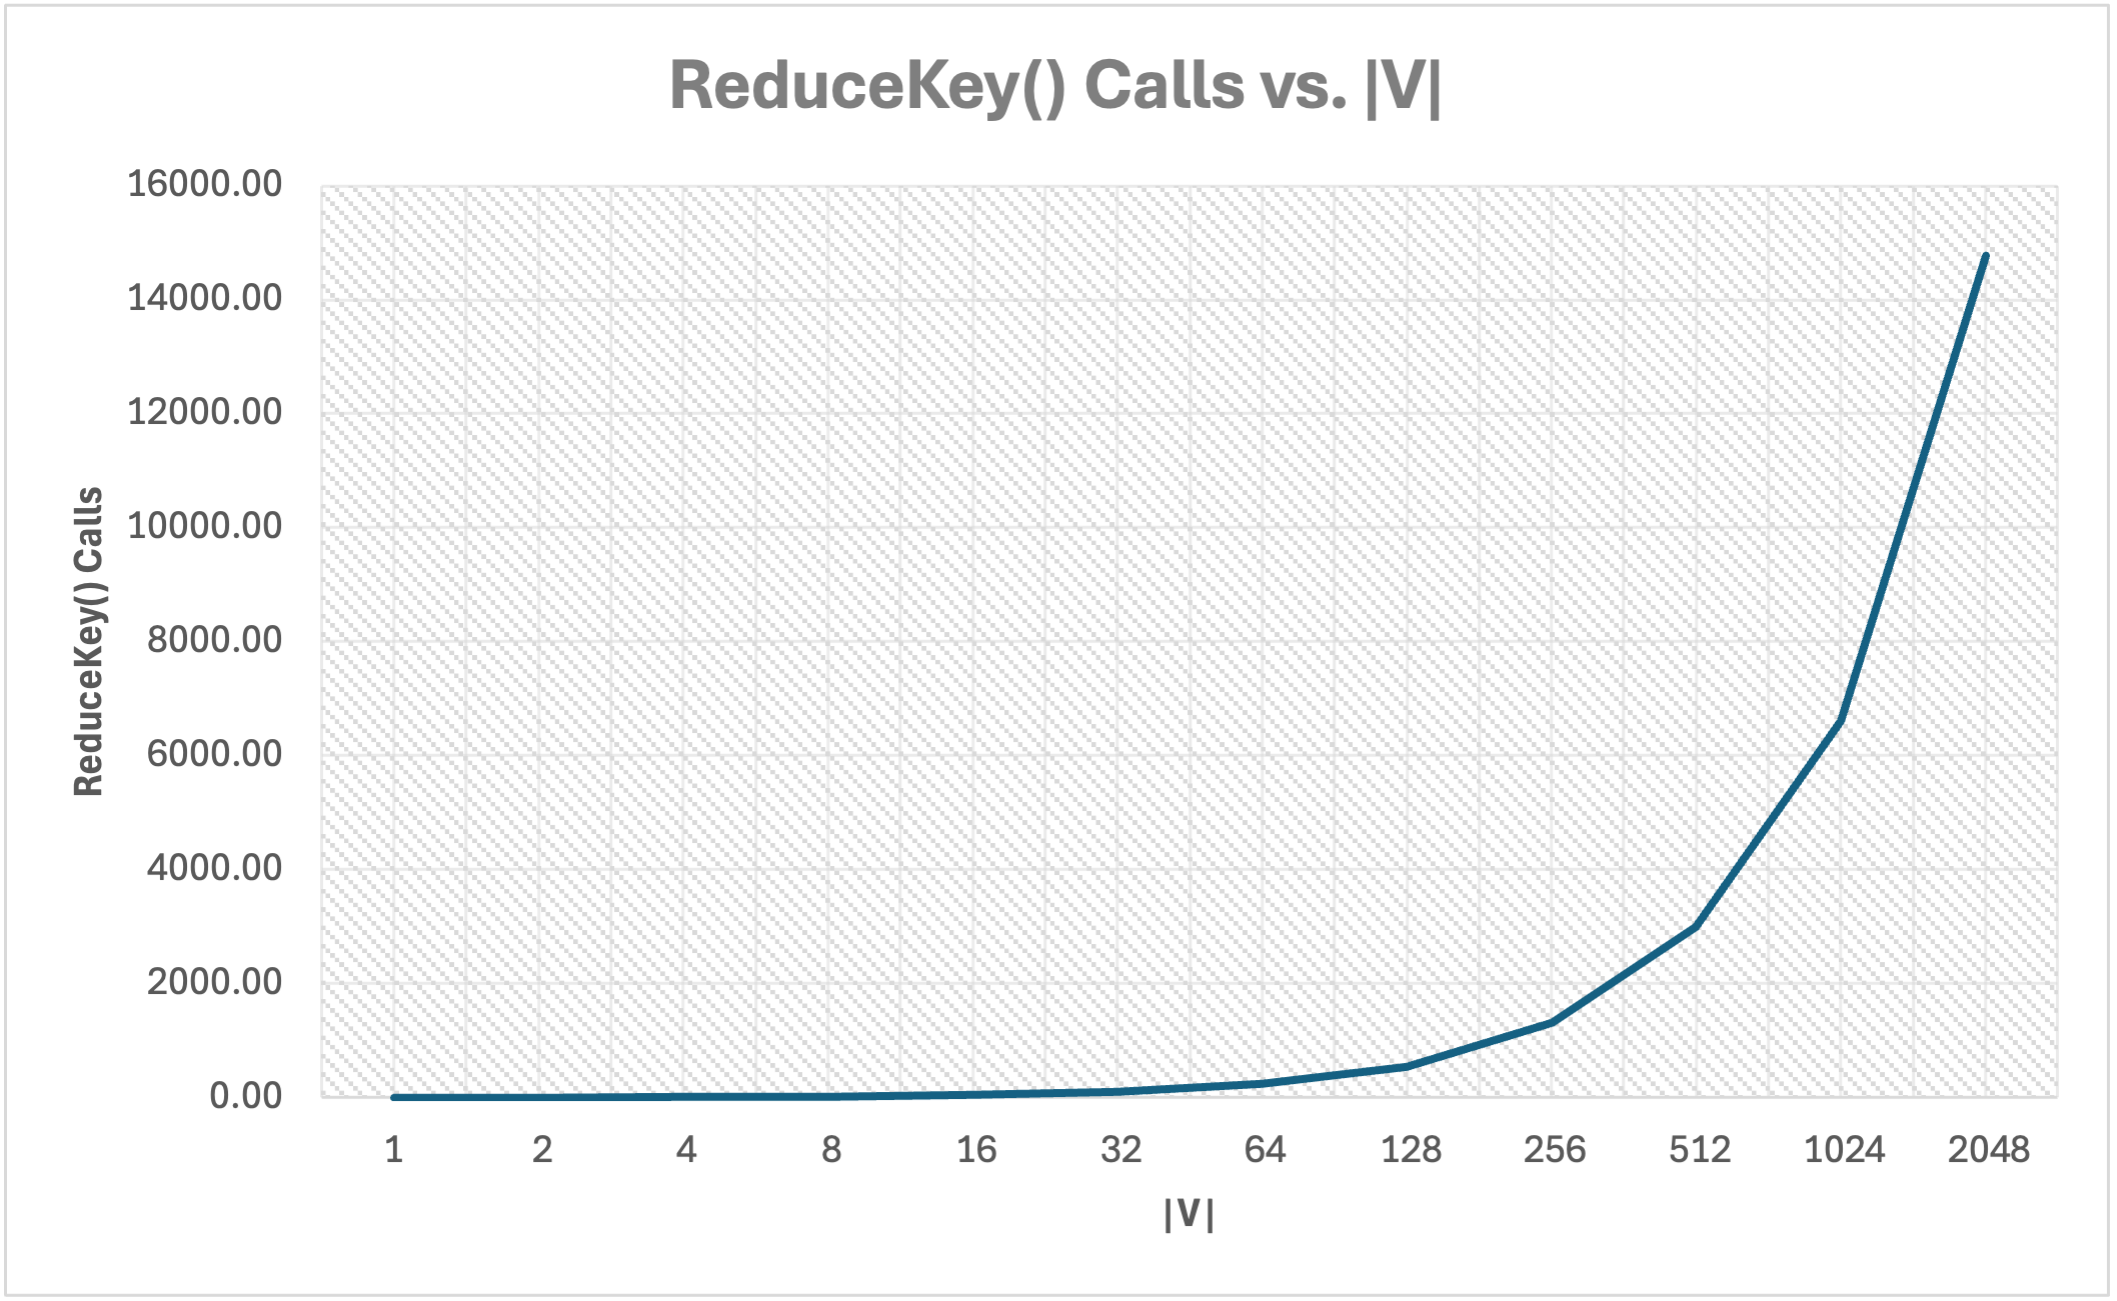
\includegraphics[width=0.45\textwidth]{src/graph1.png}
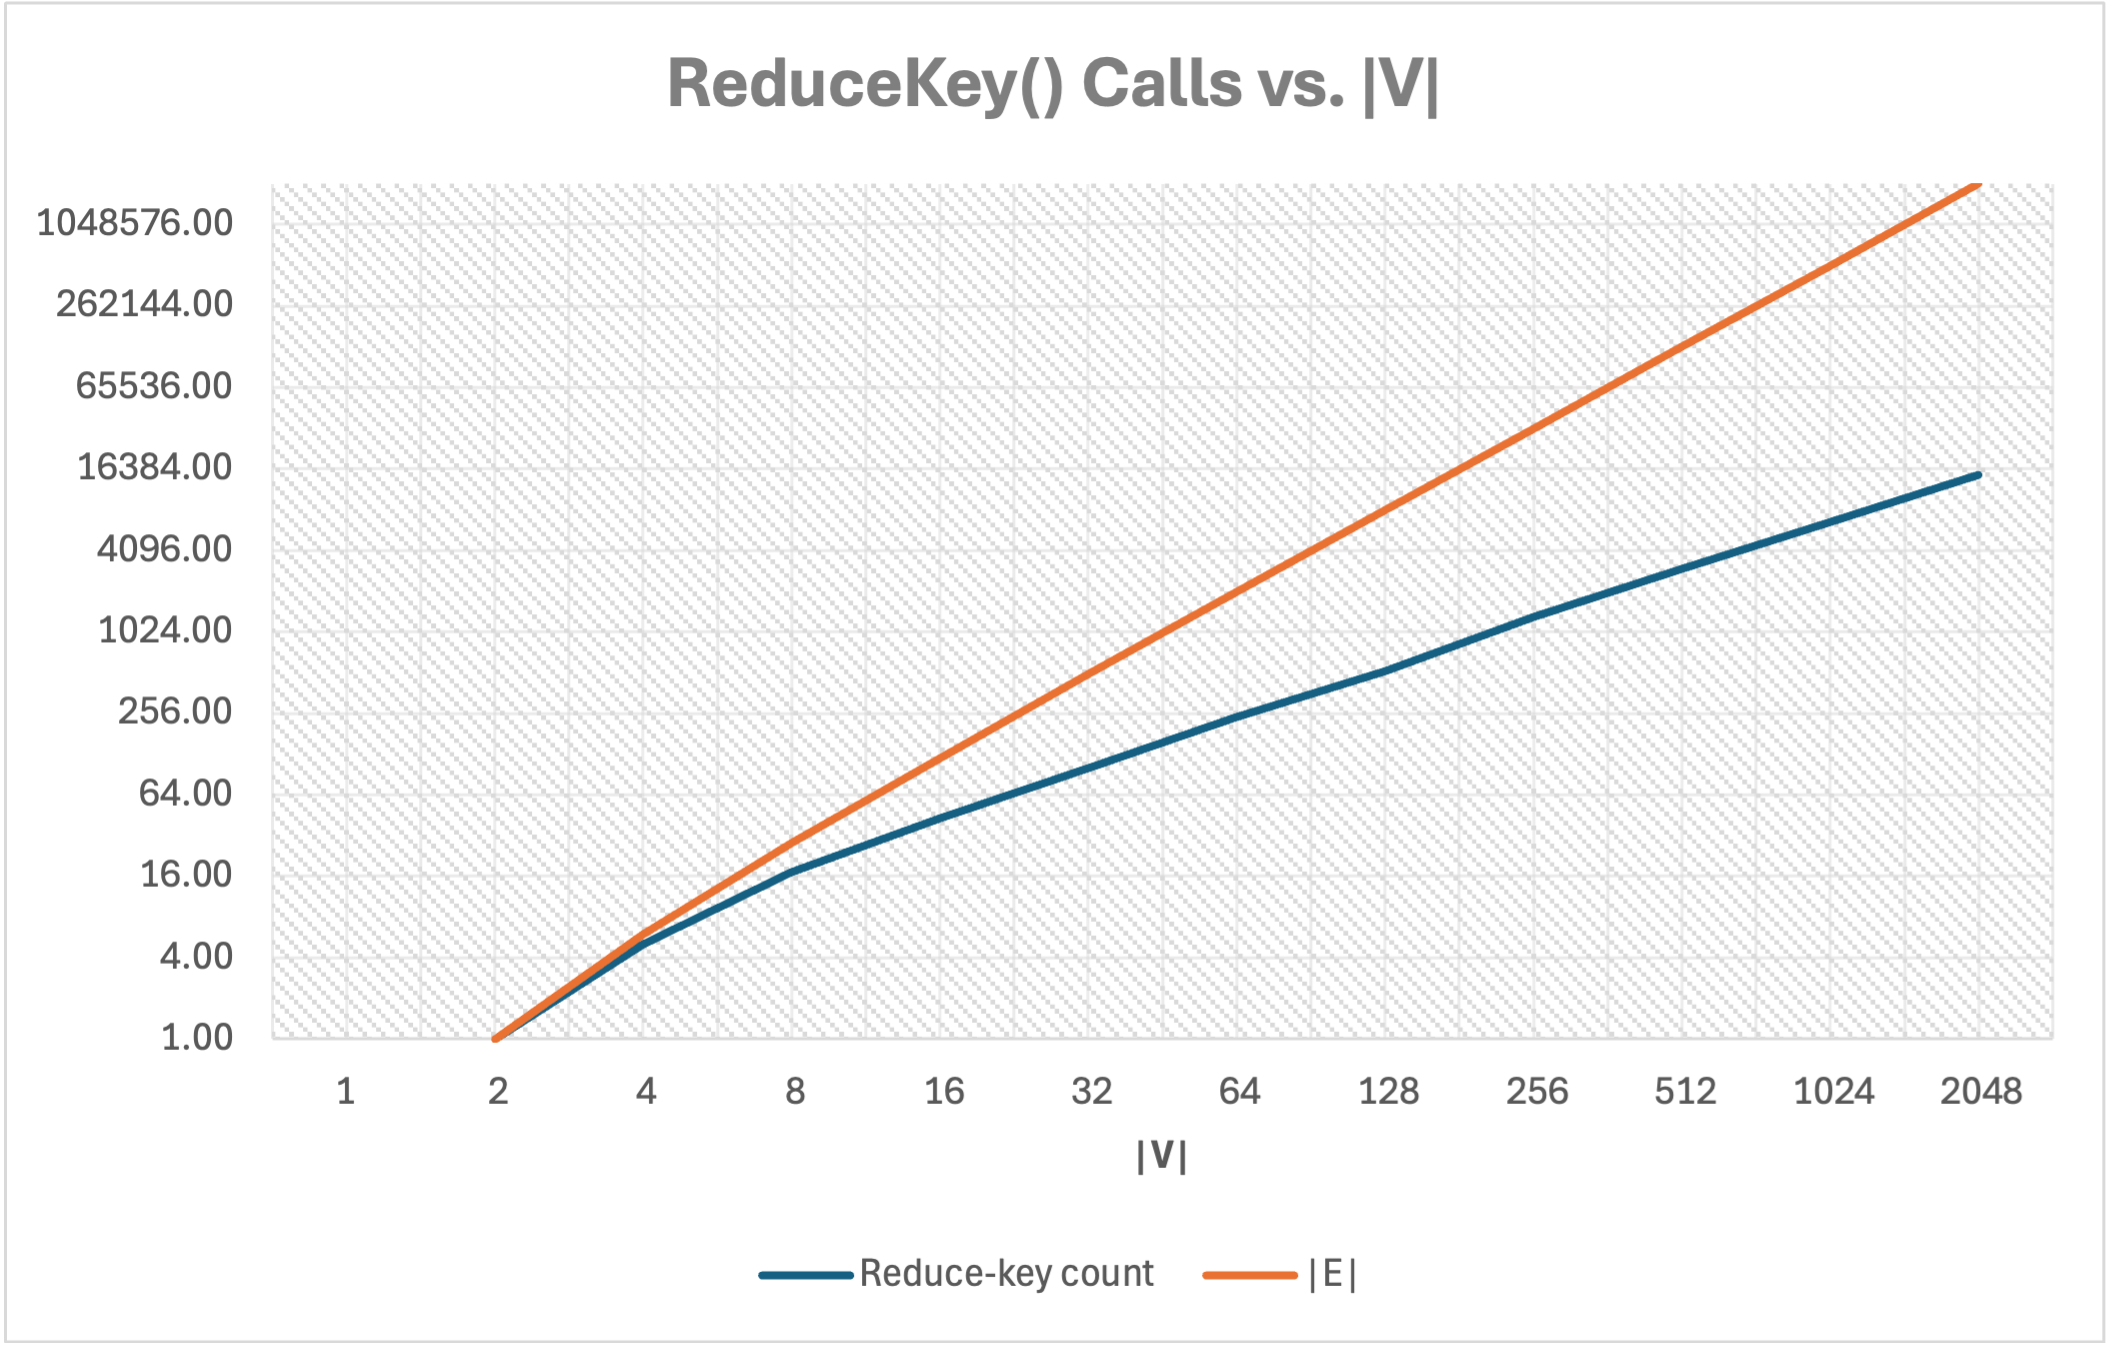
\includegraphics[width=0.45\textwidth]{src/graph2.png}

The actual number of calls to the `reduceKey()` function matches, asymptotically, the theoretical worst case bound. There are, however, consistently less actual calls to the `reduceKey()` function than the theoretical worst case number of calls.

They match asymptotically because the average case and the worst case number of calls of `reduceKey()` are the same using a min heap implementation. Specifically, both are proportional to the number of edges in the graph, \(|E|\) (\(|E| = \frac{|V| \cdot (|V| - 1)}{2}\), for a complete graph). 

In practice, the number of calls is less than the worse-case, maximum numbers of calls, since `reduceKey` is only called when a new shortest path is found, which is not true for every edge.



\end{enumerate}
\end{document}

